\section{Técnica de evaluación de fiabilidad}
La evaluación de la fiabilidad es de suma importancia para el desarrollo de sistemas críticos, ya
que permite identificar que aspectos del comportamiento del sistema juega un papel importante
\citep{FTDesign}.

Como lo indica \cite{FTDesign} existen dos enfoques convencionales para evaluar fiabilidad:
\begin{enumerate}
 \item Modelado de un sistema en la fase de diseño.
 \item Aseguramiento del sistema en la fases finales de desarrollo (testing).
\end{enumerate}

La evaulación de la fiabilidad tiene dos aspectos. En primer lugar se tiene una \textit{evaluación
cualitativa} que permite identificar, clasificar y medir modos de fallas, o eventos combinacionales
que puedan provocar una falla. El otro aspecto es la \textit{evaluación cuantitativa}, la cual
permite evaluar en términos de probabilidad los atributos de la fiabilidad
(Sección \ref{sec:atributos_de_la_fiabilidad}), disponibilidad, seguridad.

\section{Medidas comunes de fiabilidad}
Las medidas de fiabilidad más comunes son las siguientes: failure rate, tiempo medio a la falla,
tiempo medio de reparación y tiempo medio entre fallas.

\subsection{Failure rate}
Failure rate $\lambda$ es el número esperardo de fallas por unidad de tiemp \citep{FTDesign}. Es
usual utilizar la dimensión \textit{fallas/horas}.

Generalmente, $\lambda$ se encuentra a nivel de componente. Para conocer el failure rate del
sistema completo, se puede realizar (a groso modo) una sumatoria de los $\lambda$ de los
componentes que integran el sistema. $$\lambda=\sum_{i=1}^{n} \lambda_i$$.

La evolución de $\lambda$ a través del tiempo, no tiene el mismo comportamiento tanto para \ac{HW} como para \ac{SW}
Si se devide el ciclo de vida de un sistema en las siguientes fases: mortalidad prematura (I), vida útil (II), desgaste (II) \citep{FTDesign}
se aprecia, para el caso del \ac{HW}, lo que se denomina \textit{curva de la bañera} la cual puede observarse en la Figura \ref{fig:bathtub_curve}.
En una primera fase, $\lambda$ decrese, ya que a través de los procesos de testing se van descubriendo y resolviendo los errores. Luego se da un periodo de estabilización.
Y al final, el \ac{HW} sufre el paso del tiempo, y se desgasta, aumentando la tasa de fallas.

\begin{figure}[h]
 \centering
 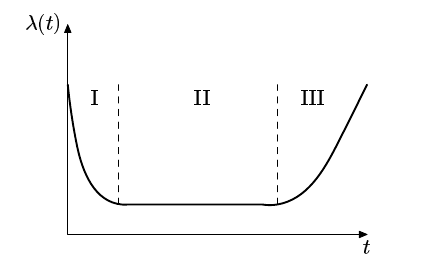
\includegraphics[scale=0.5]{images/Marco_teorico/bathtub_curve.png}
  \caption{Failure rate de HW vs tiempo }
\label{fig:bathtub_curve}
\end{figure}

Para el \ac{SW} es totalmente diferente. En primer lugar cuando se realiza una actualización, se aumenta la complejidad, como así también la probabilidad de fallas,
con ello el failure rate. Otra diferencia sustancia con el \ac{HW} es que el \ac{SW} no se desgasta con el tiempo. En la Figura \ref{fig:Failure_rate_software}
se aprecia $\lamda$ a través de tiempo. Esta curva suele llamarse \texit{curva serrucho}.

\begin{figure}[h]
 \centering
 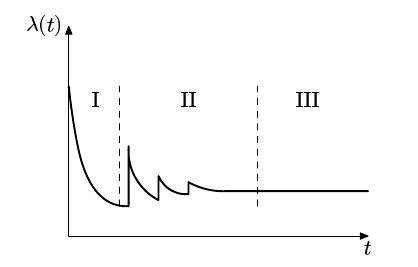
\includegraphics[scale=0.5]{images/Marco_teorico/Failure_rate_software.png}
  \caption{Failure rate SW vs tiempo }
\label{fig:Failure_rate_software}
\end{figure}
